\documentclass{article}
\usepackage{amsmath}
\usepackage{amssymb}
\usepackage{enumitem}
\usepackage{algorithm}
\usepackage{listings}
\usepackage{color,xcolor}
\usepackage[T1]{fontenc}
\usepackage{etoolbox}
\usepackage{multicol}
\usepackage{geometry}
\usepackage[colorlinks=true,linkcolor=blue,urlcolor=red,bookmarksopen=true]{hyperref}
\usepackage{tikz, pgfplots, tkz-euclide,calc}
    \usetikzlibrary{patterns,snakes,shapes.arrows,3d,patterns.meta,angles,quotes}
    \geometry{
        total = {160mm, 237mm},
        left = 25mm,
        right = 35mm,
        top = 30mm,
        bottom = 30mm,
      }

\usepackage{tcolorbox}
     \tcbuselibrary{listings,skins}

\newcommand{\enter}{\raisebox{-1.8pt}{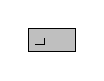
\begin{tikzpicture}[scale=0.3]
    \draw[thin,fill=lightgray] (0,0) rectangle (2,1);
    \draw (0.3,0.3) -- (0.7,0.3)--(0.7,0.6);     
\end{tikzpicture}}}

\definecolor{HIMAmuda}{HTML}{01D1FD}
\definecolor{HIMAtua}{HTML}{02016A}
\definecolor{HIMAabu}{HTML}{CBCBCC}
\definecolor{pgray}{rgb}{0.5,0.5,0.5}
\definecolor{pblue}{rgb}{0.13,0.13,1}
\definecolor{pgreen}{rgb}{0,0.5,0}
\definecolor{pred}{rgb}{0.9,0,0}
\definecolor{pgrey}{rgb}{0.46,0.45,0.48}
\definecolor{pcyan}{HTML}{D4EFFC}
\definecolor{lblue}{HTML}{00AEEF}
\definecolor{input}{HTML}{AAE1FA}
\definecolor{bg}{rgb}{0.95, 0.95, 0.92}
\definecolor{vscode}{HTML}{282A36}
\definecolor{PastelGreen}{HTML}{77DD77}

\newcommand{\inputscan}[1]{\raisebox{0pt}[1pt]{\colorbox{darkgray}{#1}}}

\usepackage{listings}

\lstdefinestyle{Liang}{
language=Java,
showspaces=false,
showtabs=false,
breaklines=true,
showstringspaces=false,
breakatwhitespace=true,
commentstyle=\color{pgray},
keywordstyle=\color{pblue},
stringstyle=\color{pgreen},
basicstyle=\small\ttfamily,
frame=single,
backgroundcolor=\color{pcyan},
escapeinside={(*}{*)},}

\lstdefinestyle{output}{
    language=Java,
    backgroundcolor=\color{vscode},
    basicstyle=\small\ttfamily\color{white},
    frame=none,
    escapeinside={(*}{*)},
    showspaces=false,
    showtabs=false,
    breaklines=true,
    showstringspaces=false,
    breakatwhitespace=true,
    keywordstyle=\color{white},
    }

\lstdefinestyle{standard}{
    language=Java,
    showspaces=false,
    showtabs=false,
    breaklines=true,
    showstringspaces=false,
    breakatwhitespace=true,
    commentstyle=\color{pgray},
    keywordstyle=\color{pblue},
    stringstyle=\color{pgreen},
    basicstyle=\small\ttfamily,
    frame=single,
    backgroundcolor=\color{bg},
    escapeinside={(*}{*)},}
\lstset{style=Liang}

\newtcblisting{RunCode}[1][enhanced,drop shadow]{
    arc=0pt, outer arc=0pt,
    boxsep=1pt,
    boxrule=2pt,
    auto outer arc,
    colback=vscode,
    colframe=bg,
    listing only, 
    listing style=output,
    title=\color{black}Ex. Output,
    #1
    }

\newtcolorbox{hint}[1][]{
    colback=PastelGreen!5!white, 
    colframe=PastelGreen!75!black,
    fonttitle=\bfseries, 
    colbacktitle=PastelGreen!85!black,
    enhanced, 
    attach boxed title to top left={yshift=-2mm}, 
    title=Hint,
    #1
}

\newtcolorbox{req}[1][]{
    colback=lblue!5!white, 
    colframe=lblue!75!black,
    fonttitle=\bfseries, 
    colbacktitle=lblue!85!black,
    enhanced, 
    attach boxed title to top left={yshift=-2mm}, 
    title=Input,
    #1
}

\newtcolorbox{out}[1][]{
    colback=HIMAtua!5!white, 
    colframe=HIMAtua!75!black,
    fonttitle=\bfseries, 
    colbacktitle=HIMAtua!85!black,
    enhanced, 
    attach boxed title to top left={yshift=-2mm}, 
    title=Output,
    before upper=\renewcommand\thempfootnote{\Roman{mpfootnote}},
    #1
}

\renewcommand{\thesubsection}{\arabic{subsection}}
\newcommand{\R}{\mathbb{R}}
\newcommand{\Z}{\mathbb{Z}}

\title{\textbf{Tugas Pertemuan 5}}
\date{10 Oktober 2024}
\author{Dhanar A \& Fajar A}
\begin{document}

\maketitle

\begin{enumerate}
    \item Buatlah sebuah program looping seperti berikut !

    \begin{req}
        $n = 6$
    \end{req}

    \begin{RunCode}
Bentuk pertama !

1
1 2
1 2 3
1 2 3 4
1 2 3 4 5
1 2 3 4 5 6
    \end{RunCode}

    \begin{RunCode}
Bentuk kedua !

1 2 3 4 5 6
1 2 3 4 5
1 2 3 4
1 2 3
1 2
1
    \end{RunCode}

    \begin{RunCode}
Bentuk ketiga

6 5 4 3 2 1
6 5 4 3 2
6 5 4 3
6 5 4
6 5
6
    \end{RunCode}

    \begin{out}
        Lampirkan untuk iterasi manualnya !
    \end{out}
    \newpage

    \item Buatlah sebuah program yang menampilkan nilai $e$ , Aproksimasikan nilai $e$ dengan deret berikut:
    $$e = 1 + \dfrac{1}{1!} + \dfrac{1}{2!} + \dfrac{1}{3!} + \dfrac{1}{4!} + \ldots + \dfrac{1}{i!}$$

    \begin{req}
    \begin{itemize}
        \item  $i = 5, 10000 , 20000 , 100000$
    \end{itemize} 
    \end{req}

    \begin{hint}
    \begin{itemize}
        \item Karena $i! = i \times (i-1) \times \ldots \times 2 \times 1 $ , maka :
        $$\dfrac{1}{i!} = \dfrac{1}{i(i-1)!}$$
        \item Gunakan \texttt{Math.round()} untuk membulatkan bilangan
    \end{itemize}
        
    \end{hint}
    \begin{RunCode}
Masukkan nilai i : (*\inputscan{5} \enter*)
Nilai e nya adalah 2.717 
    \end{RunCode}
        \begin{RunCode}
Masukkan nilai i : (*\inputscan{10000} \enter*)
Nilai e nya adalah 2.718
    \end{RunCode}

    \begin{out}
        Lampirkan untuk iterasi manual dengan minimal 3 kali 
    \end{out}

    \newpage
    
    \item Sebuah deret geometri memiliki bentuk umum :
    $$S_n = a + ar + ar^2 + \ldots + ar^{n-1}$$
    Buatlah sebuah program yang menhitung jumlah dari deret tersebut , lewatkan suku-suku yang bernilai negatif

    \begin{req}
        \begin{itemize}
            \item $-5\leq \text{a} \leq 5 \quad a \in \R $
            \item $-1 < \text{r} < 1 \quad r \in \R , \quad r \neq 0$
        \end{itemize}
    \end{req}
    \begin{hint}
        \begin{itemize}
            \item Gunakan \texttt{Math.pow()} untuk memangkatkan bilangan
            \item Gunakan \texttt{continue} untuk melewatkan suku negatif
            \item Hitung sampai suku ke-10
        \end{itemize}
    \end{hint}
        \begin{out}
            \begin{itemize}
                \item $S_n:=$ Jumlah deret\footnote{Cukup tampilkan 3 angka di belakang koma}\\
                $S_n\geq 0,\quad d\in\R$
            \end{itemize}
        \end{out}
        \begin{RunCode}
Masukkan a : (*\inputscan{3} \enter*)
Masukkan r : (*\inputscan{0.5} \enter*)
Jumlah deret geometri nya adalah 5.994
        \end{RunCode}

        \begin{RunCode}
Masukkan a : (*\inputscan{-3} \enter*)
Masukkan r : (*\inputscan{-0.5} \enter*)
Jumlah deret geometri nya adalah 1.998
        \end{RunCode}

\end{enumerate}

\end{document}
